\documentclass{ximera}

%\addPrintStyle{..}

\begin{document}
	\author{Bart Lambregs}
	\xmtitle{Golven en kenmerken}{}
    \xmsource\xmuitleg

	%%%\section{Golven \& kenmerken}
	
	Golven kunnen we volgens hun kenmerken indelen in een paar categoriën. Zo kunnen we een onderscheid maken tussen \emph{mechanische} en \emph{elektromagnetische} golven. Mechanische golven hebben een (elastisch\footnote{De vervorming in het medium kan zich maar voortzetten van zodra het lichaam te vervormen is en dus elastisch is. Er moeten immers krachten tussen de verschillende plaatsen van het medium aanwezig zijn.}) medium nodig om zich in te verplaatsen -- het is de storing in het medium die de golf vormt. Elektromagnetische golven daarentegen hebben geen medium nodig. Het zijn de elektrische en de magnetische veldenvectoren die golven.\footnote{Ook de recentelijk gemeten zwaartekrachtgolven moeten tot de categorie behoren van golven die geen medium nodig hebben. Het zijn rimpelingen van de ruimte-tijd zelf.}
	\begin{image}
	
	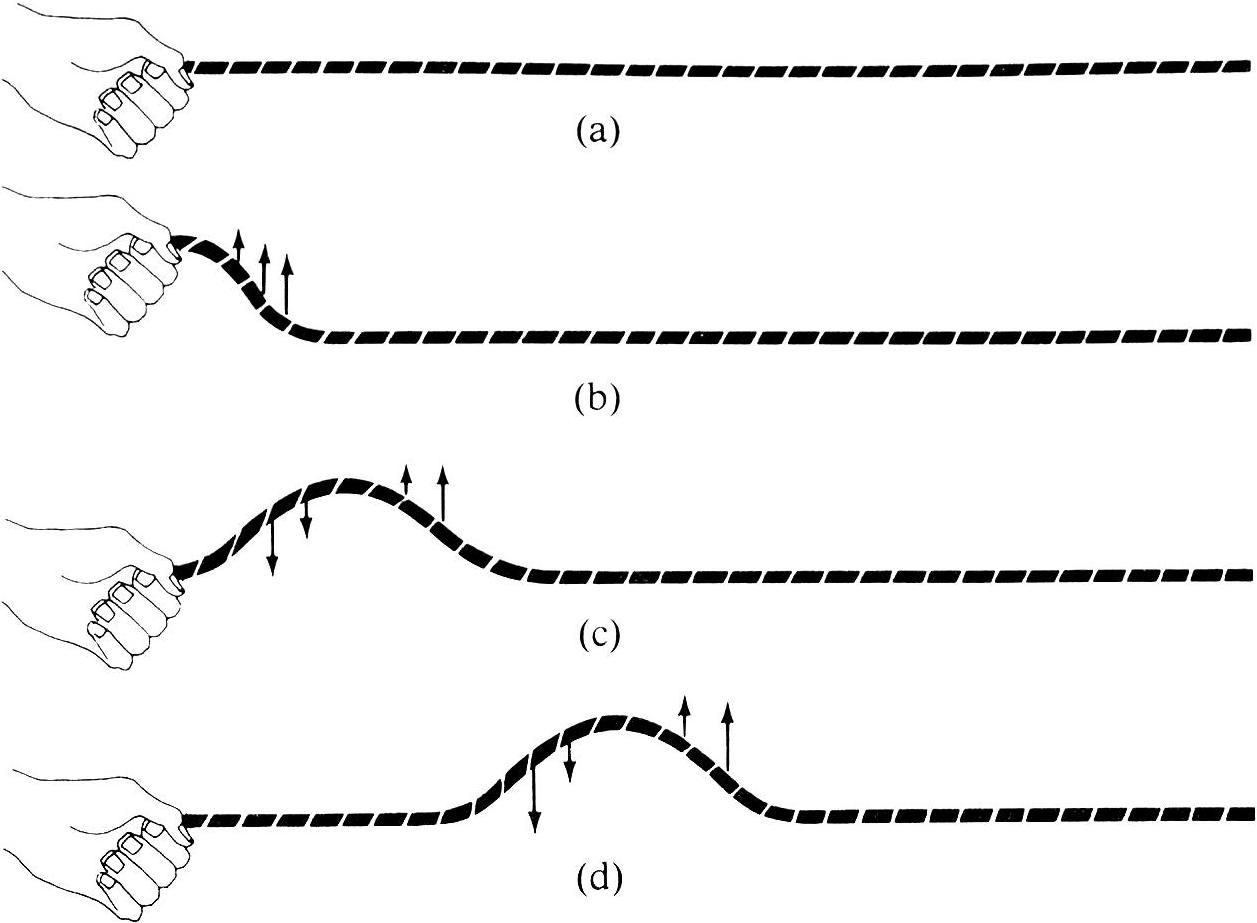
\includegraphics[width=0.7\textwidth]{elasticiteit_medium}
	\end{image}
	\captionof{figure}{\textit{Een golfpuls die zich voortplant in een touw. De pijlen geven de snelheid van deeltjes in het touw weer.}}
	
	%%%\newline
	%%%\newline
	Golven kunnen \emph{transversaal} of \emph{longitudinaal} zijn. Bij een transversale golf gebeurt de beweging van de deeltjes van het medium loodrecht op de voortplantingsrichting van de golf. Zo krijg je transversale golven wanneer je het uiteinde van een touw heen en weer slingert. Ook licht is een transversale golf. Hier trilt dus niet het medium maar is het de oriëntatie van de elektrische of magnetische veldvector die loodrecht staat op de voortplantingsrichting. Bij een longitudinale golf bewegen de deeltjes van het medium in de richting evenwijdig met de voortplantingsrichting. P-golven bij een aardbeving zijn hiervan een voorbeeld (i.t.t. S-golven, die zijn transversaal). Ook geluid bestaat uit een longitudinale golf. Zo plant geluid zich in de lucht voort doordat de luchtmoleculen tegen elkaar botsen. 
	Er zijn nog andere soorten golven zoals \emph{oppervlaktegolven}, \emph{tweedimensionale} en \emph{driedimensionale} golven. Deze zullen we hier met momenten kort behandelen.
	\begin{image}
	
	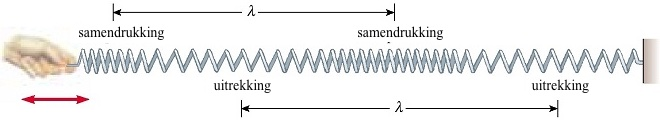
\includegraphics[width=0.9\textwidth]{longitudinaal_veer}
	\end{image}
	\captionof{figure}{\textit{Een longitudinale golf in een opgegespannen veer. De verplaatsingen van de spiralen zijn in de richting van de zich voortplantende golf. Elke samendrukking wordt gevolgd door een uitrekking.}}
	%%%\newline
	%%%\newline
	Als een de bron van een golf voortdurend blijft trillen, spreken we van een \emph{continue golf} of lopende golf. Als je slechts een enkele verstoring hebt die zich voortplant, spreken we van een \emph{puls}. We zullen hier in de regel over continue golven spreken.
	%%%\newline
	%%%\newline
	Om een golf te kunnen beschrijven, hebben we een paar karakteristieke grootheden. Zo kunnen we bij een continue golf spreken over de \emph{golflengte}. De golflengte $\lambda$ van een golf is de kortste afstand tussen twee punten die in fase trillen. Deze is gemakkelijk terug te vinden als de afstand van top tot top\footnote{In de ruimtelijke voorstelling van de golf kan je over golftoppen, -pieken of -kammen spreken tegenover golfdalen. Voor een longitudinale golf spreken we over samendrukkingen of verdichtingen versus uitrekkingen of verdunningen.}. De golflengte is dus de periode voor de golf in de ruimte zoals de `periode' $T$ de periode is van een trilling in de tijd. Voor een continue golf is de \emph{periode} de tijd die een deeltje nodig heeft om een volledige trilling te doorlopen. Omdat dit evenzeer de tijd is die de storing nodig heeft om de golflengte af te leggen, hebben we de volgende eenvoudige maar belangrijke formule voor de snelheid waarmee de golf zich voortplant -- de \emph{golfsnelheid} of fasesnelheid:
	\begin{equation*}
	v=\frac{\lambda}{T}=\lambda\cdot f
	\end{equation*}
	%De eenheid van golflengte is dan ook de meter, daar waar die voor de periode de seconde is.
	In de regel zullen we golven behandelen waarvoor de snelheid onafhankelijk is van de frequentie of golflente van de golf.\footnote{Is de snelheid wel afhankelijk van de frequentie, dan spreken we over dispersie. Dit verschijnsel doet zich onder andere voor bij licht dat door een prisma gaat. De snelheid voor verschillende kleuren en dus frequenties is verschillend waardoor je een regenboogeffect krijgt. De snelheid bepaalt immers de mate van breking.} In dat geval zijn golflengte en frequentie dus omgekeerd evenredig.
	%%%\newline
	%%%\newline
	Voor een golf kan je naast de golfsnelheid nog een andere snelheid beschouwen. De deeltjes van het medium kunnen namelijk harmonisch trillen zodat hun snelheidsverloop helemaal verschillend is van de constante golfsnelheid waarmee de storing zich voortplant. De onderstaande figuur verduidelijkt dit.
	\begin{image}
	
	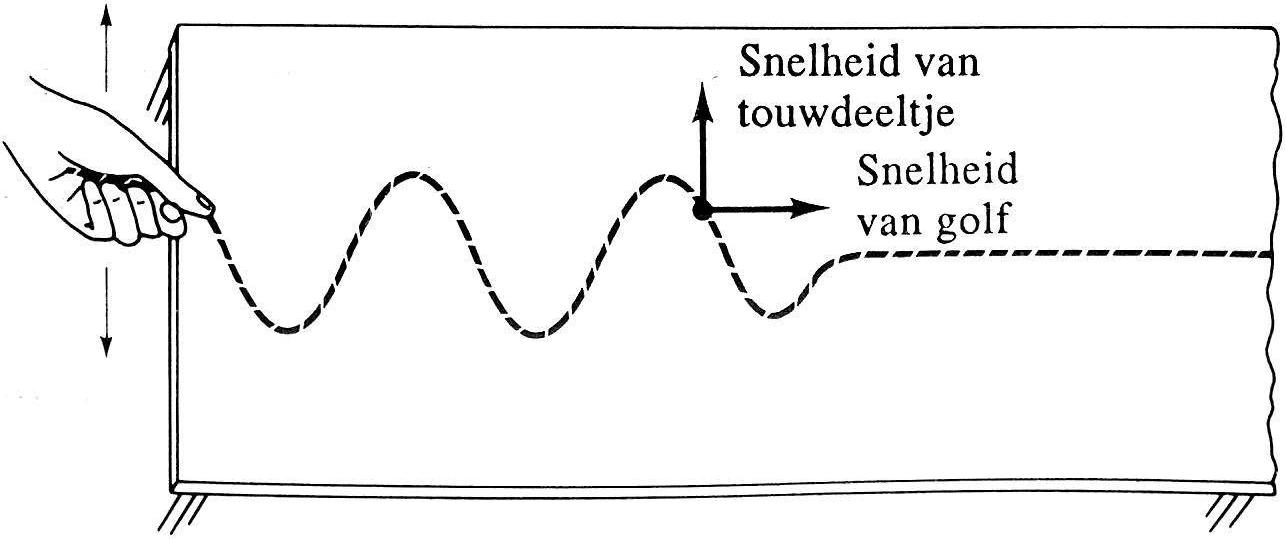
\includegraphics[width=0.9\textwidth]{golf_vs_deeltjessnelheid}
	\end{image}
	\captionof{figure}{\textit{De golf beweegt naar rechts terwijl de deeltjes van het touw oscilleren.}}
	
	%- overdracht van energie
\end{document}
